
%%%%%%%%%%%%%%%%%%%%%%%%%%%%%%%%%%%%%%%%%%%%%%%%%%%%%%%%%%%%%%%%%%%%%
% LaTeX Template: Project Titlepage Modified (v 0.1) by rcx
%
% Original Source: http://www.howtotex.com
% Date: February 2014
% 
% This is a title page template which be used for articles & reports.
% 
% This is the modified version of the original Latex template from
% aforementioned website.
% 
%%%%%%%%%%%%%%%%%%%%%%%%%%%%%%%%%%%%%%%%%%%%%%%%%%%%%%%%%%%%%%%%%%%%%%

\documentclass[12pt]{article}
\usepackage[utf8]{inputenc}
\usepackage[a4paper]{geometry}
\usepackage[myheadings]{fullpage}
\usepackage{enumitem}
\usepackage{fancyhdr}
\usepackage{lastpage}
\usepackage{graphicx, wrapfig, subcaption, setspace, booktabs}
\usepackage[T1]{fontenc}
\usepackage[font=small, labelfont=bf]{caption}
\usepackage{fourier}
\usepackage{amsmath}
\usepackage[protrusion=true, expansion=true]{microtype}
\usepackage[english]{babel}
\usepackage{sectsty}
\usepackage{url, lipsum}
\usepackage{titlesec}
\usepackage{diagbox}
\usepackage{pdfpages}

\usepackage{listings}
\usepackage{color}

\usepackage{longtable}
\newcolumntype{P}[1]{>{\centering\arraybackslash}p{#1}}
\newcolumntype{M}[1]{>{\centering\arraybackslash}m{#1}}

\definecolor{dkgreen}{rgb}{0,0.6,0}
\definecolor{gray}{rgb}{0.5,0.5,0.5}
\definecolor{mauve}{rgb}{0.58,0,0.82}

\lstset{frame=tb,
  language=C++,
  aboveskip=3mm,
  belowskip=3mm,
  showstringspaces=false,
  columns=flexible,
  basicstyle={\small\ttfamily},
  numbers=none,
  numberstyle=\tiny\color{gray},
  keywordstyle=\color{blue},
  commentstyle=\color{dkgreen},
  stringstyle=\color{mauve},
  breakatwhitespace=true,
  breaklines=true,
  tabsize=2
}

\newcommand{\HRule}[1]{\rule{\linewidth}{#1}}
\onehalfspacing
\setcounter{tocdepth}{5}
\setcounter{secnumdepth}{5}
\inputencoding{utf8}

\titleformat{\paragraph}
{\normalfont\normalsize\bfseries}{\theparagraph}{1em}{}
\titlespacing*{\paragraph}
{0pt}{3.25ex plus 1ex minus .2ex}{1.5ex plus .2ex}


%-------------------------------------------------------------------------------
% HEADER & FOOTER
%-------------------------------------------------------------------------------
\pagestyle{fancy}
\fancyhf{}
\setlength\headheight{15pt}
\fancyhead[L]{António Pedro Araújo Fraga}
\fancyhead[R]{Cranfield University}
\fancyfoot[R]{Page \thepage\ of \pageref{LastPage}}
%-------------------------------------------------------------------------------
% TITLE PAGE
%-------------------------------------------------------------------------------

\begin{document}

\title{ \fontsize{40}{90} \textsc{Test Plan}
		\\ [2.0cm]
		\HRule{0.5pt} \\
		\LARGE \textbf{Simulated computing system}
		\HRule{2pt} \\ [0.5cm]
		\normalsize \today \vspace*{5\baselineskip}}

\date{}

\author{
		\textbf{António Pedro Araújo Fraga} \\
		\textbf{Student ID: 279654} \\ 
		\textbf{Cranfield University} \\
		\textbf{M.Sc. in Software Engineering for Technical Computing
		} }

\maketitle
\thispagestyle{empty}
\newpage
\tableofcontents
\thispagestyle{empty}
\newpage

%-------------------------------------------------------------------------------
% Section title formatting
\sectionfont{\scshape}
\titleformat{\section}
{\normalfont\huge\bfseries}{\thesection}{1em}{}
\titleformat{\subsection}
{\normalfont\large\bfseries}{\thesubsection}{1em}{}
\titlespacing*{\section}
{0pt}{5.5ex plus 1ex minus .2ex}{4.3ex plus .2ex}
\titlespacing*{\subsection}
{0pt}{5.5ex plus 1ex minus .2ex}{4.3ex plus .2ex}
%-------------------------------------------------------------------------------

%-------------------------------------------------------------------------------
% BODY
%-------------------------------------------------------------------------------

%-------------------------------------------------------------------------------
% Introduction
%-------------------------------------------------------------------------------

\section*{Test Plan Identifier}
\addcontentsline{toc}{section}{Test Plan Identifier}

Simulated Computing System, Fraga


\section*{Product Overview}
\addcontentsline{toc}{section}{Product Overview}
\par This system will be developed under two modules, \textbf{Software Testing and Quality Assurance} and  \textbf{Requirements Analysis and System Design} at \textbf{Cranfield University}. 
\par It is supposed to simulate a computer system which runs jobs of several sizes. The jobs last between \textbf{one second} and \textbf{sixty four hours}, assigning them with a category of \textbf{Short}, \textbf{Medium}, \textbf{Large} or \textbf{Huge}. The system shall be capable of scheduling a job running time on a basis of a \textbf{First Come, First Served} methodology, analysing what is the correct time to run a job every time a submission is made. The simulation must generate a set of informations regarding the pretended outputs. These outputs are dependent of inputs values that will be established in the beginning of the simulation.


\par The application is going to be used by the IT department, modelling the behaviour of a real computing platform and exploring alternative accounting strategies.

\par The system shall attend functional and non-functional requirements. Most of functional requirements shall be tested at the \textbf{Unit \& Integration level}, whereas non-functional requirements shall be tested at a higher level.

\section*{Testing Synopsis}
\addcontentsline{toc}{section}{Testing Synopsis}

\subsection*{Items to be tested}
\addcontentsline{toc}{subsection}{Items to be tested}

\begin{itemize}  
\item Coding standards
\item Compatibility 
\item Functional 
\item Reliability
\end{itemize}

\subsection*{System Requirements}
\addcontentsline{toc}{subsection}{Features and Functions to test}

These requirements are specified in the \textbf{System Requirements Specification} document.

\subsection*{References \& Standards}
\addcontentsline{toc}{subsection}{References \& Standards}

This test plan is based on the \textbf{IEEE 829 format}, regarding to a test plan outline. 

\pagebreak

\section*{Types of Testing}
\addcontentsline{toc}{section}{Types of Testing}

\subsection*{Acceptance Testing}
\addcontentsline{toc}{subsection}{Acceptance Testing}

\begin{figure}[!htb]
  \centering
  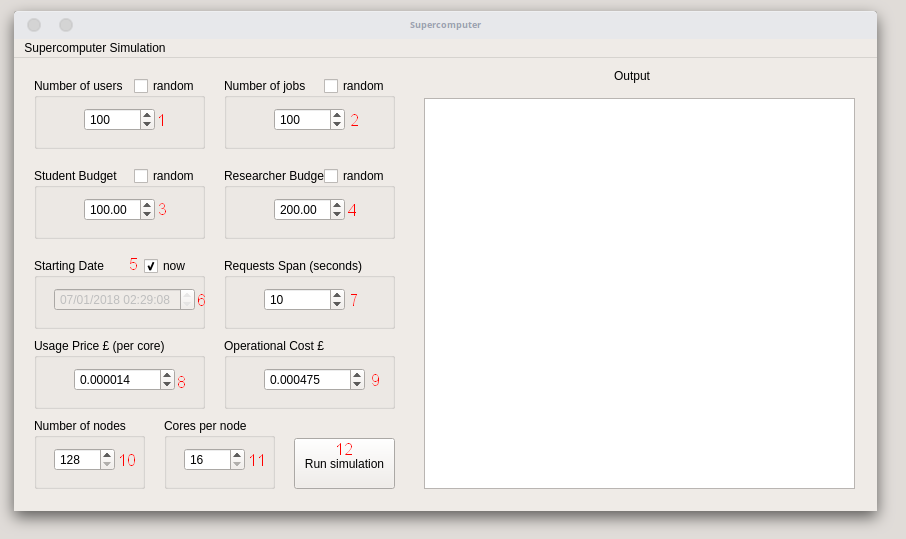
\includegraphics[width=\linewidth]{GUI.png}
\end{figure}

\begin{itemize}  
\item \textbf{AT01} A user is able to change the number of simulated users by changing the spin box labelled with \textbf{1}.

\item \textbf{AT02} A user is able to change the number of simulated jobs by changing the spin box labelled with \textbf{2}.

\item \textbf{AT03} A user is able to change the student budget by changing the spin box labelled with \textbf{3}. This spin box supports two decimal places.

\item \textbf{AT04} A user is able to change the researcher budget by changing the spin box labelled with \textbf{4}. This spin box supports two decimal places.
 
\item \textbf{AT05} A user is able to alternate between the present and a different date by hitting the checkbox labelled with \textbf{5}. If this checkbox is unchecked, the user is able to define a date by changing the date picker value labelled with \textbf{6}.

\item \textbf{AT06} A user is able to change the requests span value by changing the spin box labelled with \textbf{7}.

\item \textbf{AT07} A user is able to change the usage price per core value by changing the spin box labelled with \textbf{8}. This spin box supports six decimal places.

\item \textbf{AT08} A user is able to change the operational cost per core value by changing the spin box labelled with \textbf{9}. This spin box supports six decimal places.

\item \textbf{AT09} A user is able to change the number of nodes by changing the spin box labelled with \textbf{10}.

\item \textbf{AT10} A user is able to change the number of cores by changing the spin box labelled with \textbf{11}.

\item \textbf{AT11} A user is able to run the simulation by pressing the button labelled with \textbf{12}. The user is able to observe the simulation output in the "Output box".

\end{itemize}





\subsection*{Functional \& System Level Tests}
\addcontentsline{toc}{subsection}{Functional \& System Level Tests}

Every functional requirement will be tested with \textbf{Unit Tests}. And since the code will be developed with \textbf{C++}, \textbf{Catch}, which is an Unit Tests framework for C++, will be used. 
\textbf{Functional Tests} are the tests that will cover every single module individually. They will assure that every \textbf{single} part of the system is working as it should be. These tests will cover specific features.

\textbf{System Level Tests} will be written to test the entire system. The system, which accepts a set of inputs, will have to return a string as \textbf{Output}. This string will contain information like the \textbf{resulting price paid by the users} and the \textbf{economic balance} of the centre. This output will be tested with \textbf{regular expressions}, assuring there's a match between the actual output and the expected output. Avoiding, for instance, results like \textbf{NAN (Not A Number)} instead of an expected \textbf{floating point} value.

Code coverage will be generated by a specific tool as well. Further information will be given in the \textbf{Code Coverage} section.

\subsection*{Boundary Tests}
\addcontentsline{toc}{subsection}{Boundary Tests}

This kind of tests will included in \textbf{Unit Testing}. All boundaries are respected, so that the input values are always valid, generating valid outputs as well. 

\subsection*{Integration \& Regression Tests}
\addcontentsline{toc}{subsection}{Integration \& Regression Tests}

Integration Tests are often useful when a project is developed by a team, having different engineers developing different modules. This project will be developed in one machine, therefore testing the code on this machine can be seen as an \textbf{Integration Test}. However, a technology will run along with the \textbf{version control} system \textbf{(Travis CI)}. This technology will be responsible to run the \textbf{Unit Tests} every time there's a \textbf{merge} between repository branches. 

These repository branches, as stated in the \textbf{System Requirements Specification}, will be created every time a new \textbf{requirement} is being developed. But the version control system, will always have \textbf{two} main branches.

\begin{itemize}  
\item deployment - which will contain a version control of every accepted release. 
\item development - which will contain a version control of every pre-release (to be accepted)
\end{itemize}

When running \textbf{Unit Tests} on these branches, it will be assured that the system is running properly. 

\subsection*{Compatibility Tests}
\addcontentsline{toc}{subsection}{Compatibility Tests}

The tests and program will run in different machines running different operating systems. Every test and program execution will have to produce the correct results:

\begin{itemize}  
\item \textbf{CPU}: Intel Core i7-4750HQ, up to 3.2 GHz. \textbf{Memory}: 8GB \textbf{OS}: UNIX Elementary OS
\item \textbf{CPU}: Intel Core i7-4510U, up to 2.6 GHz. \textbf{Memory}: 8GB \textbf{OS}: UNIX Arch Linux
\item \textbf{CPU}: AMD A8-4555M APU with Radeon, 1.6 GHz. \textbf{Memory}: 8GB \textbf{OS}: Microsoft Windows 10
\item \textbf{CPU}: Intel Pentium P6000, 1.87 GHz. \textbf{Memory}: 4GB \textbf{OS}: Microsoft Windows 10
\end{itemize}

\section*{Code Coverage}
\addcontentsline{toc}{section}{Code Coverage}

\textbf{Code Coverage} will be generated by \textbf{lcov}. This tool is able to generate an \textbf{html} file with all the information about line coverage. It will indicate how many times a certain line will be executed, including the \textbf{percentage} of coverage in each file as well.

\section*{Test Schedule \& Completion Criteria}
\addcontentsline{toc}{section}{Test Schedule}

The tests shall be written whenever a requirement development is done. This will ensure that merge between branches include the new testing software along with the new functionality. Therefore, this measure will result in good quality \textbf{Integration Tests}.

\section*{Item Pass/Fail Criteria}
\addcontentsline{toc}{section}{Item Pass/Fail Criteria}

\par Every feature must be tested and approved. Unit Tests shall achieve total code coverage.

\section*{Test Plan Review}
\addcontentsline{toc}{section}{Test Plan Review}

This document will be reviewed by the \textbf{head of the IT department}. It will be assured that this document follows the \textbf{IEEE 829 format} and that it covers every bullet point of the testing procedure.

\end{document}

